\chapter{Monte Carlo experiments}\label{chapt:mc}

\section{Introduction}


\section{Quantization experiments}

\begin{figure}[H]
	\centering
	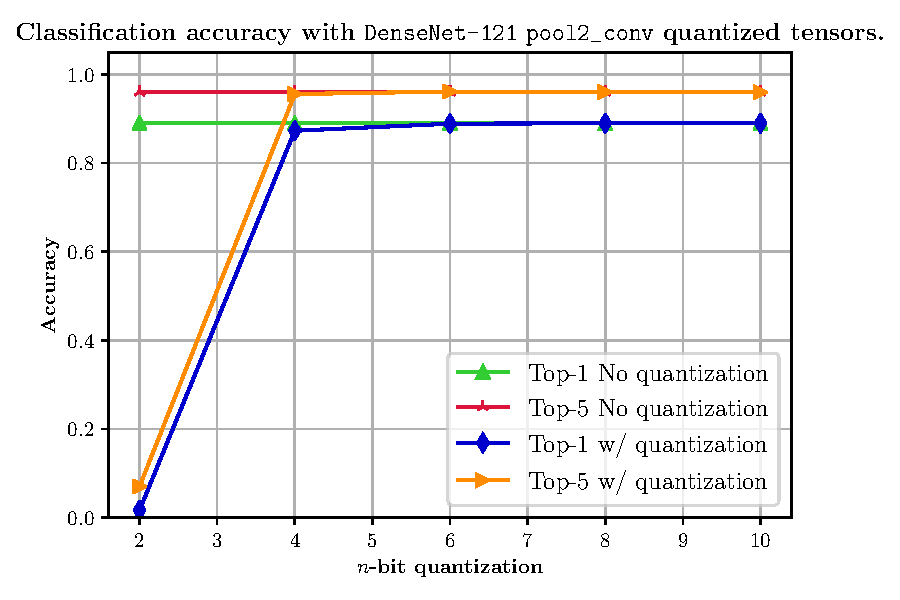
\includegraphics[scale=0.8]{Figures/quantdensenet121pool2conv.pdf}
	\caption{Quantization experiments with densenet.}
\end{figure}


\section{Lossy channel experiments}
As discussed in \ref{sec:simdescr:channel}, there are two options for imperfect channel models: random loss and Gilbert-Elliott channel models. We will focus our discussion on Gilbert-Elliott channel model experiments.



\section{Experiments with external packet traces}



\section{Summary}
This chapter discussed the mechanics of Monte Carlo experiments in DFTS. We now provide a list of example \verb|yaml| files for Monte Carlo experiments.

\begin{itemize}
	\item Quantization experiment.
	\item Gilbert-Elliott lossy channel experiment.
	\item External packet trace experiment.
\end{itemize}

